\documentclass[a4paper,12pt]{article}
\usepackage[top = 2.5cm, bottom = 2.5cm, left = 2.5cm, right = 2.5cm]{geometry}
\usepackage[T1]{fontenc}
\usepackage[utf8]{inputenc}
\usepackage{multirow} 
\usepackage{booktabs} 
\usepackage{graphicx}
\usepackage[spanish]{babel}
\usepackage{setspace}
\setlength{\parindent}{0in}
\usepackage{float}
\usepackage{fancyhdr}
\usepackage{amsmath}
\usepackage{amssymb}
\usepackage{amsthm}
\usepackage{natbib}
\usepackage{graphicx}
\usepackage{subcaption}
\usepackage{booktabs}
\usepackage{etoolbox}
\usepackage{apalike}
\usepackage{minibox}
\usepackage{hyperref}
\usepackage{xcolor}
\usepackage{tcolorbox}
\AtBeginEnvironment{align}{\setcounter{equation}{0}}
\newenvironment{solution}
  {\renewcommand\qedsymbol{$\square$}\begin{proof}[\textcolor{blue}{Solución}]}
  {\end{proof}}

\pagestyle{fancy}

\fancyhf{}

\lhead{\footnotesize Estadística 2}
\rhead{\footnotesize  Rudik Roberto Rompich}
\cfoot{\footnotesize \thepage}

\begin{document}
    \thispagestyle{empty} 
    \begin{tabular}{p{15.5cm}}
    \begin{tabbing}
    \textbf{Universidad del Valle de Guatemala} \\
    Departamento de Matemática\\
    Licenciatura en Matemática Aplicada\\\\
   \textbf{Estudiante:} Rudik Roberto Rompich\\
   \textbf{E-mail:} \textcolor{blue}{ \href{mailto:rom19857@uvg.edu.gt}{rom19857@uvg.edu.gt}}\\
   \textbf{Carné:} 19857
    \end{tabbing}
    \begin{center}
        MM2040 - Estadística 2 - Catedrático: Eugenio Aristondo\\
        \today
    \end{center}\\
    \hline
    \\
    \end{tabular} 
    \vspace*{0.3cm} 
    \begin{center} 
    {\Large \bf HT 5
} 
        \vspace{2mm}
    \end{center}
    \vspace{0.4cm}
%---------------------------
%\begin{tcolorbox}[colback=gray!15,colframe=black!1!black,title=A nice heading]
%\end{tcolorbox}

%\fbox{lol}
%---------------------------
\section{Problema 1}
1.	M\&M/MARS, fabricante de los chocolates M\&M, realizó un sondeo nacional en el que más de 10 millones de personas dieron su preferencia para un nuevo color. El resultado de este sondeo fue el remplazo del color café claro por uno azul. En el folleto “Colors”, distribuido por el área de Asuntos del Consumidor de M\&M/Mars, la distribución de los colores de las lunetas (chocolates en forma de gragea) es la siguiente.
\begin{center}
    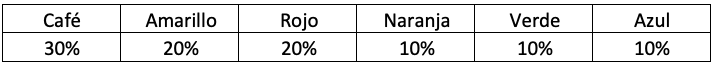
\includegraphics[scale=0.5]{images/Screen Shot 2021-05-11 at 15.46.48.png}
\end{center}
En un estudio posterior se emplearon como muestras bolsas de 1 libra para determinar si los porcentajes reportados eran válidos. En una muestra de 506 lunetas se obtuvieron los siguientes resultados.

\begin{center}
    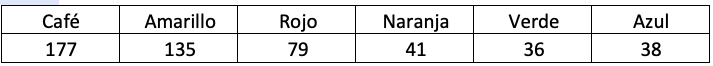
\includegraphics[scale=0.5]{images/Screen Shot 2021-05-11 at 15.47.58.png}
\end{center}
Use $\alpha$=0.05  para determinar si estos datos coinciden con los porcentajes reportados por la empresa.

\begin{solution}
Comenzamos planteando las hipótesis: 
\begin{align*}
        H_0: & 
             \text{ la población tiene una distribución multinomial con la}\\
            & \text{ probabilidad específica de cada una de las $k$ categorías.}\\
        H_a: &  
             \text{ la población no tiene una distribución multinomial con la}\\
         &\text{ probabilidad específica de cada una de las $k$ categorías.}
    \end{align*}
    
Hacemos el análisis en Geogebra: 

\begin{center}
    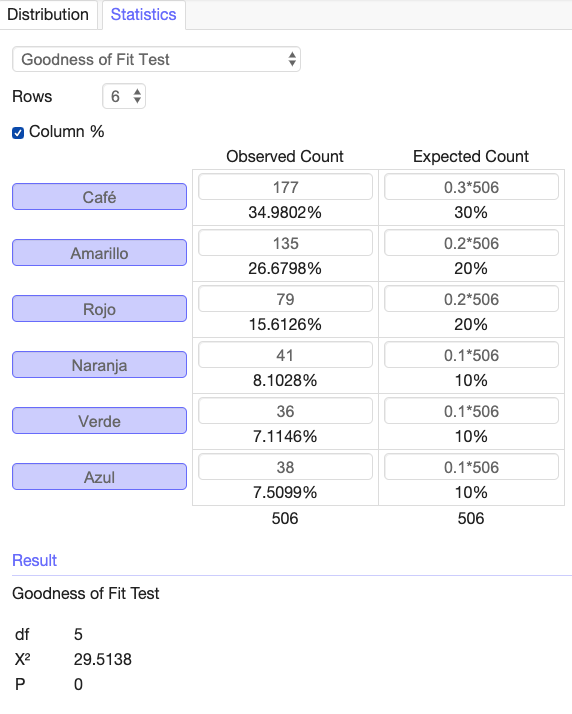
\includegraphics[scale=0.5]{images/Screen Shot 2021-05-11 at 15.53.11.png}
\end{center}
\begin{enumerate}
    \item EL valor-p es 0. 
    \item Por la prueba del valor-p, 0<0.05. Por lo tanto la $H_0$ se rechaza, es decir que la población no tiene una distribución multinomial con la probabilidad específica de cada uno de los colores respectivos.
\end{enumerate}
\end{solution}
\section{Problema 2}
2.	La National Sleep Foundation utilizó una encuesta para determinar si las horas de sueño por noche son independientes de la edad (Newsweek, 19 de enero de 2004). Las siguientes son las horas de sueño entre semana en una muestra de personas de 49 años de edad o menos, y en otra muestra de personas de 50 años de edad o más.
\begin{center}
    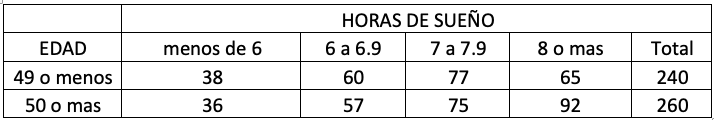
\includegraphics[scale=0.5]{images/Screen Shot 2021-05-11 at 16.01.23.png}
\end{center}


\begin{solution}
Se identifica como un problema de independencia. Se consideran las hipótesis: 
\begin{align*}
    H_0: & \text{ la variable de las columnas es independiente de la variable de las filas.}\\ 
    H_a: & \text{  la variable de las columnas no es independiente de la variable de las filas.}
\end{align*}
Haciendo el análisis en Geogebra: 
\begin{center}
    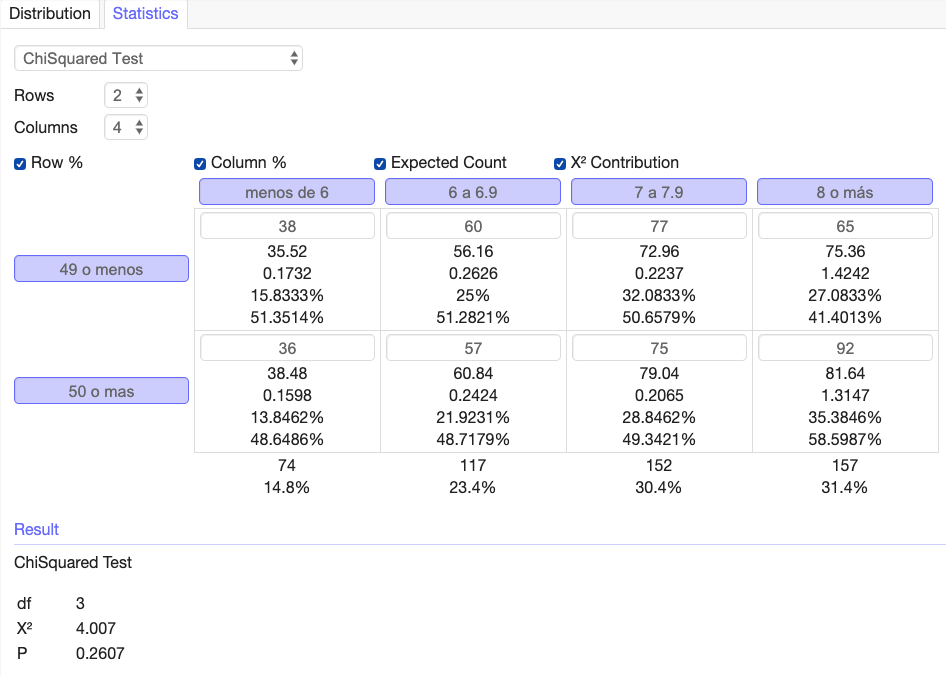
\includegraphics[scale=0.45]{images/Screen Shot 2021-05-11 at 16.07.07.png}
\end{center}
\begin{enumerate}
    \item El valor-p es 0.2607.
    \item Considerando la prueba del valor-p, 0.2607>0.05, por lo tanto, $H_0$ no se puede rechazar; las horas del sueño son independientes a la edad.
\end{enumerate}
\end{solution}

\section{Problema 3}
Se tiene la percepción de que la demanda semanal de un producto tiene una distribución normal. Aplique una prueba de bondad de ajuste y los datos siguientes para probar este supuesto. Use $\alpha$=0.1. 
\begin{center}
    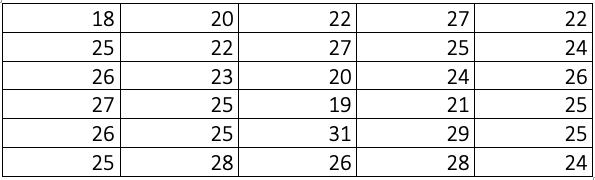
\includegraphics[scale=0.45]{images/Screen Shot 2021-05-11 at 16.16.56.png}
\end{center}

\begin{solution}
En un vistazo inicial, la distribución se ve así: \begin{center}
    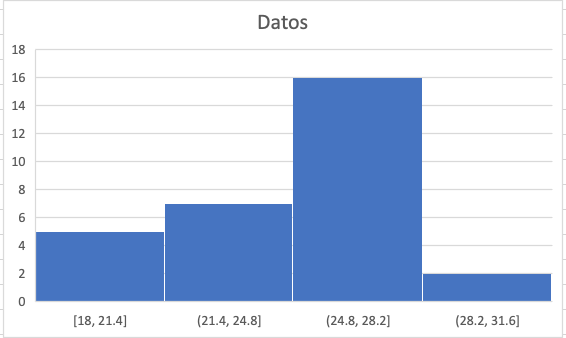
\includegraphics[scale=0.45]{images/Screen Shot 2021-05-11 at 16.29.48.png}
\end{center}
Las hipótesis se formulan como: 
\begin{align*}
    H_0: & \text{ la población tiene una distribución normal.}\\ 
    H_a: & \text{  la población no tiene una distribución normal.}
\end{align*}

Se propone dividir los datos en 5 secciones de 20\% cada una. Es decir, que ahora tenemos: 
\begin{center}
    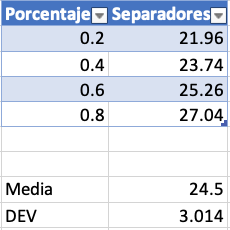
\includegraphics[scale=0.45]{images/Screen Shot 2021-05-11 at 16.38.17.png}
\end{center}

Es decir, que se tiene: 
\begin{center}
    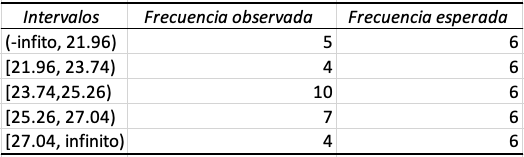
\includegraphics[scale=0.45]{images/Screen Shot 2021-05-11 at 16.45.10.png}
\end{center}

Gráficamente: 

\begin{center}
    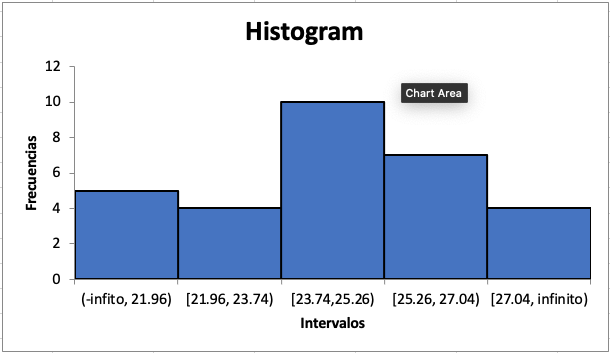
\includegraphics[scale=0.45]{images/Screen Shot 2021-05-11 at 16.45.43.png}
\end{center}

Haciendo el análisis en Geogebra:
\begin{center}
    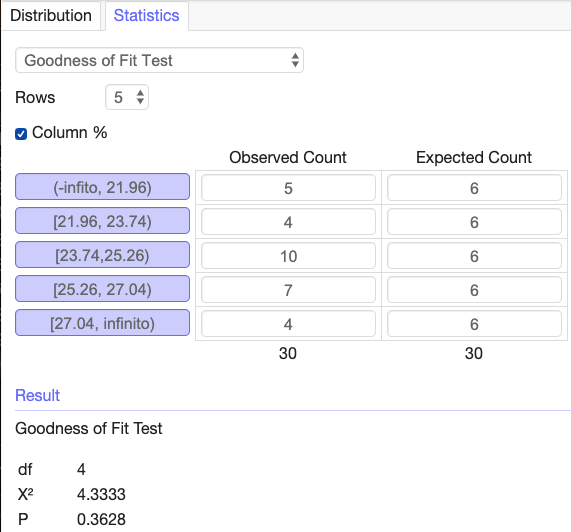
\includegraphics[scale=0.45]{images/Screen Shot 2021-05-11 at 16.52.55.png}
\end{center}
\begin{enumerate}
    \item El valor-p es 0.3628. 
    \item Por lo tanto, considerando la prueba del valor-p: 0.3628>0.1. Es decir que $H_0$ se acepta, entonces los datos tienen una distribución normal con una significancia de 0.1. 
\end{enumerate}
\end{solution}

\section{Problema 4}

Se cree que el número de llamadas telefónicas que llegan por minuto al conmutador de una empresa tiene una distribución de Poisson. Use $\alpha$=0.1   y los datos de la página siguiente para probar este supuesto. 
\begin{center}
    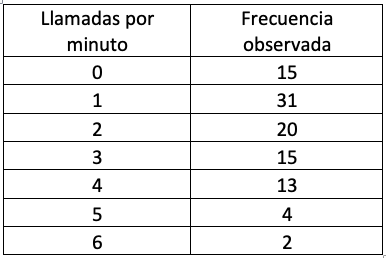
\includegraphics[scale=0.45]{images/Screen Shot 2021-05-11 at 17.00.54.png}
\end{center}
\begin{solution}
Primero, se hacen los cálculos pertinentes con Excel, usando la distribución de Poisson definida como: 

$$f(x)=\frac{\mu^xe^{-\mu}}{x!}$$

Por lo cual, se tiene: 
\begin{center}
    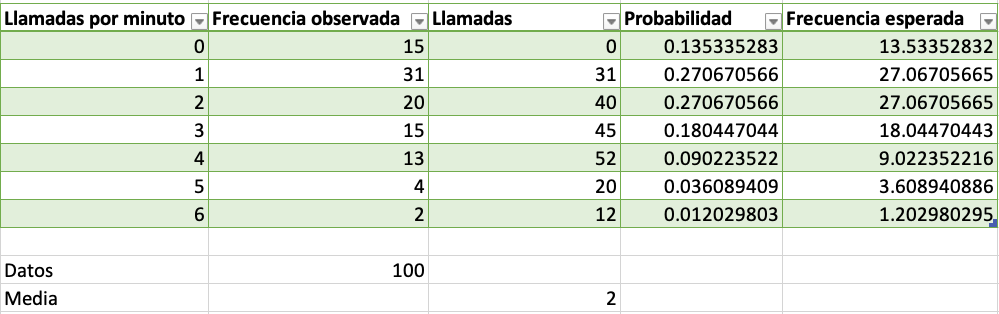
\includegraphics[scale=0.45]{images/Screen Shot 2021-05-11 at 17.19.28.png}
\end{center}

Definimos las hipótesis: 

\begin{align*}
    H_0: & \text{ la población tiene una distribución de Poisson.}\\ 
    H_a: & \text{  la población no tiene una distribución de Poisson.}
\end{align*}

Usando Geogebra: 
\begin{center}
    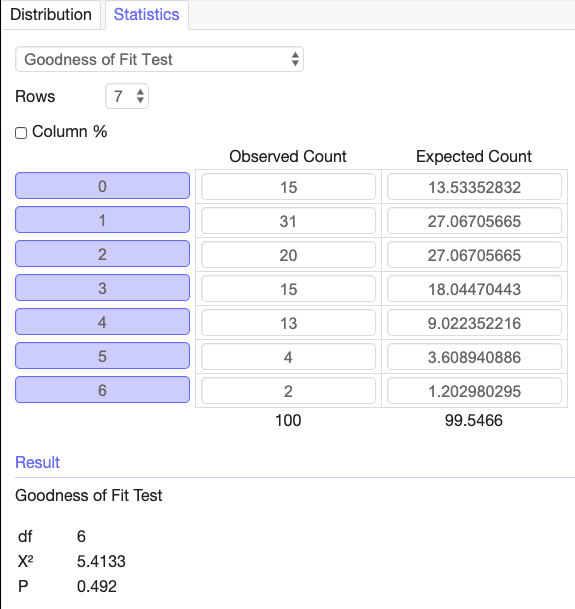
\includegraphics[scale=0.45]{images/Screen Shot 2021-05-11 at 17.21.02.png}
\end{center}

\begin{enumerate}
    \item El valor-p es 0.492. 
    \item Por el método del valor-p: $0.492>0.1$; por lo que $H_0$ no se rechaza. Por lo tanto, podemos concluir que los datos sí se ajustan a una distribución de Poisson.
\end{enumerate}
\end{solution}

%---------------------------
%\bibliographystyle{apalike}
%\bibliography{sample.bib}

\end{document}